\documentclass[phd]{ntuthesis}

\usepackage{times}
\usepackage{verbatim}
\usepackage{color}
\usepackage{url}
\usepackage{graphicx}
\usepackage{array}

% Using the tex-text mapping for ligatures etc.
\defaultfontfeatures{Mapping=tex-text}

% Set the default fonts
\setmainfont{Times New Roman}
\setCJKmainfont{微軟正黑體}

% Your information goes here
% author: Tz-Huan Huang [http://www.csie.ntu.edu.tw/~tzhuan]

% ----------------------------------------------------------------------------
% "THE CHOCOLATE-WARE LICENSE":
% Tz-Huan Huang wrote this file. As long as you retain this notice you
% can do whatever you want with this stuff. If we meet some day, and you think
% this stuff is worth it, you can buy me a chocolate in return Tz-Huan Huang
% ----------------------------------------------------------------------------using wearable sensors to promote human health: lesson learnt through real-world deployment

% Syntax: \var{English}{Chinese}
\university{National Taiwan University}{國立臺灣大學}
\collage{College of Electrical Engineering and Computer Science}{電機資訊學院}
\institute{Department of Computer Science and Information Engineering}{資訊工程學系}
\title{A Flexible and Extensible Wearable Platform 
to Promote Health Applications}{促進健康應用發展之具彈性及可擴充性之穿戴式平台}
\author{Cheng-Yuan Li}{李爭原}
\studentid{D99922035}
\advisor{Hao-Hua Chu, Ph.D.}{朱浩華 博士}
\year{2016}{105}
\month{July}{7}
\day{29}


\begin{document}

\frontmatter

\makecover

%\makecertification

%%\begin{acknowledgementszh}
%感謝\ldots
%\end{acknowledgementszh}

\begin{acknowledgementsen}
I'm glad to thank
\end{acknowledgementsen}

%\begin{abstractzh}
%\end{abstractzh}

\begin{abstracten}
\noindent

  
\end{abstracten}

%\begin{comment}
%\category{I2.10}{Computing Methodologies}{Artificial Intelligence -- Vision and Scene Understanding} \category{H5.3}{InformationSystems}{Information Interfaces and Presentation (HCI) -- Web-based Interaction.}

%\terms{Design, Human factors, Performance.}

%\keywords{Region of interest, Visual attention model, Web-based games, Benchmarks.}
%\end{comment}


\tableofcontents
\listoffigures
\let\cleardoublepage\clearpage  
\listoftables
\let\cleardoublepage\clearpage  

\mainmatter

% Your thesis goes here
\chapter{Introduction}
\section{Motivation}

...
%Designed for expert makers, entrepreneurs, and some industrial IoT applications
%However, it require significant engineering skill to build a workable device. There is a long developing process that embraces many cumbersome tasks including wiring, soldering and coding.
%Those platforms are flexible to choose needed modules and extensible to add more components. But those are not designed for wearable development in terms of wearability, size and functionality.


\section{Contribution}
This thesis makes the following contributions:
\begin{itemize} 
\item
...

\end{itemize}

\section{Organization}
The remainder of this thesis is organized as follows. Chapter 2 presents ...


\let\cleardoublepage\clearpage
\chapter{Background and Related Work}
This chapter starts by first surveying related wearable devices for healthcare applications that are available on the market today.
We describe technical challenges that may be faced by developers in developing and prototyping wearable devices.
Second, we describe our own case study of building a wearable device from scratch without using any platform/tool support.
We detail the amount of development effort and skill needed to motivate the need for wearable platform \& tool support.
Third, we present related application development platforms and tools in which designers and developers can use to build their devices \& applications.
We describe how BioScope addresses the issues of flexibility and extendibility lacking from these related platforms \& tools.

\section{Lesson Learned from Case Studies of Developing Health Applications}
This section discusses our lesson learned from prior case studies that we experienced the design and implementation of a wearable oral sensory system that recognizes human oral activities, such as chewing, drinking, speaking, and coughing from scratch without using any platform/tool support. 

%In these studies, we implement a sensor-embedded teeth \cite{Li2013teeth} to demonstrate the feasibility of sensing humans's oral activities with in-mouth sensor. We have yet to place a Bluetooth radio on this oral sensory unit; therefore, thin wires are used to connect the sensor board to an external data-logging device for data retrieval and power.
%As with section above, we describe the effort for manufacturing the breakout board and constructing the oral activity sensing system.
%As a proof-of-concept system, the effort of customization is relatively low comparing with building a more complicated device used in field study deployment for other applications.
%
%\begin{figure}
%\centering
%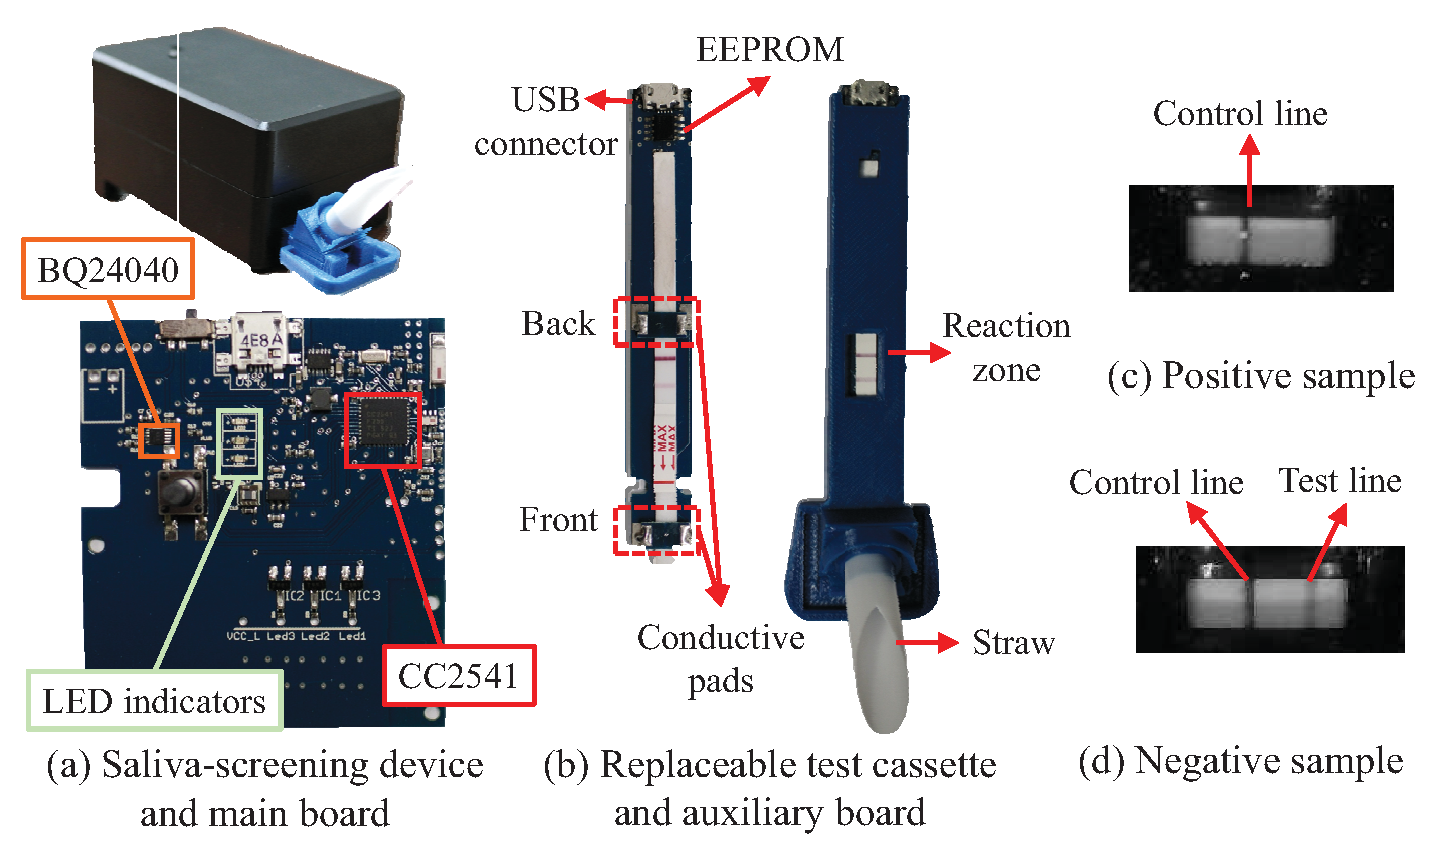
\includegraphics[width=14cm]{image/fig_ket.eps}
%\caption{(a) Saliva-screening device and main board. (b) Replaceable test cassette and auxiliary board showing (c) positive and (d) negative line patterns, which appear in the reaction zone of the cassette.}
%\label{ket_diary}
%\end{figure}
%
%Given another example (Figure \ref{ket_diary}), the KetDiary \cite{You2016Ket} is a phone-based support system to enable the self-monitoring of ketamine use by recovering patients after returning to everyday life. 
%We build a saliva-screening device to determine patient's ketamine use.
%The microcontroller triggers the camera module to capture images of the reaction zone of the test strip. When the microcontroller receives an image from the camera, a Bluetooth Low Energy (BLE) radio is used to transmit images to the patient's smartphone. 
%A phone app is built on Android platform to enable the self-monitoring and progress visualization. 
%Although, the implementation in the KetDiary is a mobile device rather than a wearable device, but this project shows that it required a lot of effort and significant engineering skill to build the system in order to use the device for a three-week study involving three ketamine-dependent patients.
%This study involves a lot of effort to implementation. First, we built a prototype to test and evaluate the sensing ability and functionality of each component using off-the-shelf development toolkit.
%After all components are validated by preliminary prototype, we customize a circuit board to make the device more compact and robust for surviving in real study. Second, the customized circuit board has a Nordic NRF51822 for BLE radio, a STMicroelectronics STM32F407 for processing image data from embedded camera, and a Texas Instruments BQ24040 for recharging a 2400-mAh Li-ion battery. Third, we design a disposable test cassette that can test users' drug use and spit action. The cases of the device and cassette are made by 3D printing. Forth, we implement and design the firmware of the device, the phone app and data server.

In order to provide a easy to use system, it requires a lot of effort and time to go through many iterations in refining modality, trouble-shooting and usability test.
In addition to the cost in building such system, developers also require significant engineering skills. However, some designers and/or developers may not be able to deal with those processes as well. Therefore, we consider that designers and/or developers should need a way to mitigate the effort and cost in the design process for building their system.

\section{Wearable Devices with Healthcare Applications}
Recently, there have been many commercial products leveraging mobile sensing and wearable technologies to promote health in people's daily life. As smartphones become ubiquitous in people's daily life, people have explored the use of smartphones together with their built-in sensors to monitor human health condition, such as basic vital-signs. For example, Instant Heart Rate \cite{Instant_Heart_Rate} is a phone application that leverages the smartphone's built-in camera and flashlight to sense a person's heart rate. Strava \cite{Strava} is a smartphone application that uses the smartphone's GPS sensor to quantify human performance of running and cycling exercises. When built-in sensors are insufficient, smartphones can also connect with external sensors, such as wearable heart rate sensors and/or cycling sensors, to collect more detailed information for further analysis of the exercise events.

Wearable devices are not only an extension of a smartphone. They can also work as a standalone device. Being wearable, it reduces people's burden of carrying additional devices. In recent years, a variety of wearable products have successfully immersed in people's daily life. Wristband is the most common form factor in wearable devices. For example, the Fitbit \cite{Fitbit} is a popular wristband device that enables people to track and monitor their physical activities. The Apple watch \cite{Apple_watch} and the Android wear \cite{Android_wear} provide wearable computing platforms to build wearable healthcare applications in the wristband form factor. Other non-wristband wearable form factors are also emerging. For examples, the Under Armour \cite{Under_armour} releases a sensor-embedded running shoe that can track and collect running metrics. The Athos \cite{Athos} is a smart apparel that monitors muscle activities and heart rate to assist training and exercise. X2 xGuard \cite{X2_xGuard, camarillo2013head} is a product that embeds sensors inside a mouth guard for tracking athletes' accumulative head impacts in contact sports, e.g.: football. The forecast for wearable devices worldwide from Gartner \cite{gartner2016wearable} shows that the market of wearable healthcare devices will experience rapid growth in the near future. 

%[What are the technical challenges these devices face that you want to put in your platform?] 

Since wearable devices are deployed and worn on humans constantly, usability plays a particularly important factor to successful people's acceptance and adoption of wearable technologies. Reaching usability goal is costly, requiring designers and/or developers to perform many iterations of prototyping, testing, analyzing, and refining to uncover and fix problems. Such development and prototyping effort can be reduced with platform support. 
%[hardware] [software]

%\section{Rapid Prototyping in HCI}
%[tool for UI]
%[3D printing]
%[]
%A proper mechanism of rapid prototyping is always an critical factor to significantly affect the progress of entire design process. Therefore, 
%some HCI researchers have paid their attention to develop better rapid prototyping .
%For example, 

\section{Rapid Prototyping for Wearable Applications}
The iterative design \cite{Nielsen:1993:IUD:618985.619982, tripp1990rapid, van2007design} between ideate, prototype and test is the most costly part in the entire design process.
The key challenge here is how to rapid prototyping in iterative design. In addition to product developers, academic researchers also have a great demand of seeking an efficient way to speed up the prototyping process. For achieving the design goal, several options can be adopted in different iteration in the design process. At the beginning of the iterative design, a low-fidelity prototype \cite{walker2002high} is the ideal tool to rapidly examine the feasibility, check the usability and refine the ideal with minimum cost of building prototype. However, low-fidelity prototype may not be able to test the functionality on certain aspects. For example, we attempted to develop a wearable oral sensory system that recognizes human oral activities related to health \cite{Li2013teeth}. For examining its feasibility, it requires building a wearable device integrated with the sensor. Therefore, people always demand a useful tool that contains electronic and/or mechanical components in the design process. In the subsequent subsections, we describe the related works of rapid prototyping for wearable applications.



\subsection{Integrated Design Devices}
Developers, designer and researchers would like to develop a wearable application with uncomplicated process and without significant engineering skill to work with it, such as wiring, soldering, coding and so on. For non-engineering background users, an off-the-shelf device would be a better choice. For examples, activPAL \cite{activPAL} equips motion sensor and storage for collecting human's physical activity. Shimmer \cite{Shimmer} is a device that integrates various types of sensors, storage, wireless connectivity and software for accessing the device. The Mercury \cite{Lorincz:2009:MWS:1644038.1644057} is an example that uses Shimmer in their study for high-fidelity motion analysis of patients being treated for neuromotor disorders. The HealthPatch \cite{vitalconnect} is a bandage-like wearable device that embedded ECG sensor, accelerometer and temperature sensor to track human's health.
Smart phone is also a versatile device that integrated many sensors. 
Eric C. Larson et.al. \cite{Larson:2011:APP:2030112.2030163} leverage the microphone on the smart phone carried in shirt pocket or using a neck strap for preserving the cough activity.
But a fixed design can only offer limited functionalities and meet the needs of limited applications. Once the user need an extra function or different form factor, it can not satisfy the need of developing new application and service. Thus, the people may be willing to pay more cost and effort for better prototyping their design.


\subsection{Prototyping platforms}
Several tools can help people to easily prototype a device for developing and testing a design. For example, the Arduino \cite{Arduino} is an open-source platform that provides easy-to-use hardware and software for making electronic device. It also has the version, e.g.: Arduino Gemma, that targets the user for developing wearable application. Arduino is a successful platform that you can easily get many resources to prototype your idea including plenty of compatible sensors, actuators, feedback components and software libraries.
The Intel Edison \cite{IntelEdison} presents a development kit that offers high computational performance and wireless connectivities including Wi-Fi and Bluetooth. Through a breakout board, it can connect other components as well as the Arduino.
The Xadow \cite{xadow} is another platform which is similar to Arduino. It adopts a well-defined connector and cable to simplify the process of connecting the components. Thus, the user is not necessary to worry about the wiring for connecting components in pin-to-pin fashion and the robustness of those wires.
The Arduino provides not only the hardware boards in its platform but also the IDE and many software libraries to support writing codes and uploading binary codes to the board. 
The Processing \cite{Processing} is an IDE to program the codes running on the PC side for communicating with a device, processing data and building 2D/3D visualization. The Arduino IDE and Processing are both open-source. Therefore, there have many third-party libraries which users can leverage in their development.
The microcontroller adopted by the Arduino has only limited computational capability and types of IO interface. 
The Arm mbed \cite{mbed} is an web-based IDE that can support for programming different devices from different manufacturers which adopt the microconotrllers with the Arm Cortex-M architecture.

Several works focus on simplifying software development process of building application.
Many applications rely on machine learning algorithms to construct their functions.
The Weka \cite{Weka} from University of Waikato integrates several popular machine learning algorithms that can be used in prototyping phase. 
But such type of tool still requires a lot of basic knowledge of data processing and machine learning. Several researchers present the mechanism to reduce the threshold for first-time users. For example, the Jigsaw \cite{Jigsaw2010} proposes a system for simplifying the effort of building the applications that require continuous sensing on a mobile phone. The users can use this platform to build an application that need to recognize every day activities using a mobile phone with a proper balance between performance and resource demand.
Choudhury et. al. \cite{Mobile_Sensing_Platform} present a wearable sensing platform designed for constructing activity-aware system that can support ubiquitous computing applications. The wearable sensing platform implements a wearable device that equips Bluetooth radio, flash storage, microphone, light sensor, accelerometer, digital compass, barometer and humidity/temperature sensor. This study also is involved in developing a software framework running on their device for data logging, feature processing and activity recognition.
The d.tool \cite{dtool} demonstrates a platform that facilitates the iterative process between design, test and analysis for prototyping information appliances with low threshold. A plug-and-play hardware board allows prototyping device by choosing needed components including button input, accelerometer, digital compass, LED, LCD screen, speaker and so on. An IDE on the PC supports the iterative process for programming prototype, testing builded functions and reviewing the data from testing.
Since many applications on wearable devices need to work with a mobile phone together. Chi et. al. presents the Weave \cite{Weave2015} that provides a web-base IDE with library to enable programming and testing for constructing behavior interactions and UI layouts across wearable and mobile devices. 

However, those platforms may not be friendly to the users who are not engineering background. They still need to pay a great effort to learn how to coding and prototyping using those platforms. After a prototype device is constructed and programed, its wiring mechanism is not robust in connecting component or its form factor is not suitable in wearable while use in testing. Then troubleshooting would be a considerable cost in iterative design process. When they leap over the prototyping phase and advance to a finished device. The effort in prototyping phase is wasted due to the constructed device and the codes can not be reuse in their finished device that should have further considerations, e.g.: compact and power saving. 

\subsection{Customization in HCI}
After several iterations of prototyping a system of the wearable application in low-fidelity and medium-fidelity prototypes, the next step is to build a high-fidelity prototype for conducting a field trial and further refine the design. 
In product development, the implementation of the wearable system will involve with a great cost and effort in customization before launching the application and service to the market.
In some cases, low-fidelity prototype may not be able to satisfy the requirement of design goal and validate the design hypothesis. 
Therefore, many HCI studies customize their wearable system in order to have a workable and robust device used in field trial or to better demonstrate their design and concept.
For examples, the mPuff \cite{mPuff:2012:MAD:2185677.2185741} introduces a chest-worn device for detecting smoking behavior using motion, heart rate, respiration and galvanic skin response sensors.
The MARS \cite{Mokaya:2013:MMA:2461381.2461406} customizes wearable devices with inertial sensors to recognize whole body movement.
However, a number of studies for wearable application \cite{mPuff:2012:MAD:2185677.2185741, Lane:2015:ZCD:2742647.2742672, Mokaya:2013:MMA:2461381.2461406, Thompson:2015:DHA:2750858.2807536, Mokaya:2015:MVB:2750858.2804258, Lorincz:2009:MWS:1644038.1644057, Yatani:2012:BWA:2370216.2370269} use common components in their customized device. The effort, cost and time to revise the prototype in customization will further increase with more iterations they go through. 

\subsection{Modular Design: Flexible and Extensible}
Modular design is a design concept that separates each functional partition of the system as a module and standardizes the communication interface between modules to enable flexibility and extensibility.
Each module can be reuse to reduce the cost in customization. A modularized system can easily add new functionality without re-design entire system to shorten developing process.
Google Ara \cite{GoogleAra} and LG G5 \cite{LGG5} are flexible and extensible smart phones that allow users to make the choice of modules for building a smart phone as their need. The modular design also enables easily to extend new module, update existing module and replace broken module.
The Nascent \cite{Nascent} allows users to build a ready-to-use electronic device using modular components such as speaker, inertial sensor and microphone, which has a similar quality to a commercial product.

Recently, modular design also emerged in wearable area.
Similar to modular smart phones, the BLOCKS \cite{BLOCKS} is a modular smartwatch that lets users to tailor the features as they needed. It contains several modules that can function on the wrist, such as temperature sensor, ECG, GPS, camera, NFC, gesture control and so on. 
The Vigekwear \cite{Vigekwear} is a developing kit that offers micro and modularized components including BLE microcontroler, inertial sensors, temperature sensor, barometer, heart rate sensor and OLED display.
This developing kit aims for allowing users to develop an application on the wrist.

The concept has been widely explored in product manufacturing to discuss the tradeoff between modular design integrated design\cite{schilling2000toward, ulrich1995role}. 
In addition to making a modular design in manufacturing phase, i.e., each component is modularized physically, modularization also can be done in design phase. For example, the Altium Designer \cite{AltiumDesigner} is a PCB design software that can encapsulate a part of circuit as a module. Thus, the designer can rearrange the module to create different configurations and variants. However, there still is a great effort to wire each module in pin-to-pin fashion.

Those examples show that the modular design can be a useful concept to benefit rapid prototyping for developing wearable applications. 
In our BioScope platform, we leverage the concept of the modular design to enable flexibility and extendibility that can assist researcher, designer and developer for rapid prototyping their health applications. However, the design of the wearable platform has a lot of challenges that the platform can meet the needs of our users who may not have engineering background and/or related training. In the next section, we will introduce the design exploration that explore the design criteria of prototyping wearable for health applications through two focus groups and two participatory design workshops.

\let\cleardoublepage\clearpage
\chapter{Design Exploration}

The first step of iterative design for a wearable sensing platform is to understand the needs of potential users. We conducted two focus groups and two participatory design workshops to explore the needs from healthcare professionals.

\section{Focus Groups}
We conducted two focus groups to better understand the practical needs of wearable technology in clinical setting. In the first focus group, we recruited four nursing professionals and two physical therapists from National Taiwan University Hospital. In the second focus group, we recruited four nursing professionals from Taipei City Psychiatric Center (TCPC).

\subsection{Participants}
In the first focus group, we recruited four healthcare workers (four experienced nursing experts and two physiotherapists), aged from 27 to 46 years. The four experienced nursing experts had worked as registered nurses for more than three years and the two physiotherapists have worked in the Rehabilitation Department of National Taiwan University Hospital at least six years. These participants have prior experienced in oncology, cardiology, and orthopedics. Four experts in the second focus group, aged from 35 to 45 years, have worked as registered nurses for more than ten years at the Taipei City Psychiatric Center (TCPC) and specialized in providing inpatient psychiatric care for children, adolescents, geriatrics, and patients with substance abuse.

\subsection{Procedures}
The moderator of the focus group was a researcher with background in engineering. After explaining the objective of the focus group, we provide five mock-up wearable devices with different form factors to the participants. Then, the moderator asked their perceptions regarding the usability, safety, and potential applications of those form factors. The second topic of the focus group is to encourage stories with clinical scenarios that can reveal how wearable devices may benefit different healthcare applications.

\section{Participatory Design Workshops}
We conducted participatory design workshops to look for opportunities and constrains concerning the use of wearable sensing technologies in healthcare applications. Following the participatory design process \cite{Greenbaum:1992:DWC:125470, Muller:2002:PDT:772072.772138}, two workshops were held to co-design devices to assist healthcare workers in designing a wearable sensing platform.

\subsection{Participants}
Eight nursing professionals (four experienced nursing experts and four senior nursing school students), aged from 22 to 46 years, with experience in clinical nursing, were recruited. Four experienced nursing experts had worked as registered nurses for at least seven years and the four senior nursing school students had been nursing interns in hospitals for at least half a year. All participants were experienced in nursing patients in multiple medical divisions, with the main specialty spanning in divisions of oncology, pediatrics, cardiology, and orthopedics.

\subsection{Prior to a Workshop}
The nursing professionals were briefly introduced to the goal of this study and the structure of the workshop several days (about four to six days) prior to the workshop. Before attending the workshop, participants were asked to finish the pre-workshop homework similar to “homework” assignment to participants prior to each workshop in the PICTIVE project \cite{Muller:1991:PEP:108844.108896}. This pre-workshop homework involved a design sheet to help participants describe and/or sketch five potential ideas for designs of devices that used any related wearable sensing technology to assist them in resolving difficulties that they faced at work or in their daily life. Since the purpose of this pre-workshop homework was to encourage the participants to generate a wide range of designs in the workshop, the participants were not asked to evaluate the feasibility of their prototype devices for solving the described problems or to limit them in their focus on post-operative caring scenarios. This pre-workshop homework helped the participants to brainstorm a wide range of ideas and collect observations from their working or everyday life as a warm-up for the upcoming workshop.

\subsection{Procedures}
This workshop comprised of three sessions, which were (1) an engagement session, (2) a guiding session, and (3) a development session. Two participatory design workshops were held on two separate days. Each workshop lasted approximately four hours, including a half-an-hour break for lunch.

\textbf{Engagement session:} 
\newline
In the engagement session (which lasted for half of an hour), all participants introduced themselves and presented the five design ideas that they had prepared for their pre-workshop homework. While presenting a design idea, each participant stuck a design note that also described the idea on a white board. Researchers generated appropriate categories and grouped similar ideas as the participants were placing their notes. After all of the notes on the white board, researchers and participants discussed and moved the notes among categories or to a new category using the affinity diagramming method. All of the categories indicate potential directions or building blocks in the development of the solution in the final design of the workshop. 

\textbf{Guiding session:} 
\newline
In the guiding session (which lasted for half of an hour), a moderator, who was a researcher with an engineering background, introduced the sensing technologies or projects related to healthcare applications. The purpose of the workshop was explained to participants, which was to use wearable and/or environmental sensing technologies in the design of devices that can help healthcare workers in caring for post-operative patients in hospital. 

\textbf{Development session:} 
\newline
In the final developing session (which lasted two and a half hours), four participants were separated into two pairs in which each participant could share design opinions. To stir cross-disciplinary thinking within each pair, one researcher with an engineering background helped participants to identify alternative sensing technologies for use in their design work, and another researcher with a background in industrial and commercial design expressed their design scenarios using concrete storyboards. Consistent with the work-oriented participatory design process, the goal of each design was set, which was to help healthcare workers care for patients in hospitals. To assist participants in performing the design task effectively, an A3 sheet of paper with the following fields was provided; name of their solution, target user, needs of the target user, targeted sensing events and required feedback, form factor of the designed device. The first stage of the development session involved the participants discussing the name and the target user of the designed solution using categories that were obtained from the pre-workshop homework. Following the identification of the target users, the second stage involved determining the potential needs of the target user that are associated with the solution. In the third stage, the engineering researcher discussed with participants the selection of sensors and actuators for detecting targeted events or generating the required feedback in each application scenario. When the group completed its final design, the designer cooperated with the participants to finalize the form factor of the designed device by sketching an appropriate storyboard. In the final stage, each group presented their final design, about which all participants discussed and commented.

\section{Findings form Explorative Studies}
In addition to medical-background users, a team to develop an application may involve cross-disciplinary members.
The users with different background knowledge and skill levels have various requirements for prototyping. 
To better understand the needs of engineering-background users, we further conduct semi-structure interviews on 6 participants, who have experience on HCI projects (4 male and 2 female age from 22 to 33 with computer science or electrical engineering background).
The design goal of BioScope towards a flexible and extensible platform that can fit in with different types of users. We describe the design considerations for both non-engineering background and engineering background users.

For data analysis, the audio recordings of focus groups and interviews, and the video recordings of the participatory design workshops were transcribed and coded.
With lessons learned from our study and observations, we summarize the findings of design exploration for developing a wearable sensing platform as follows.

\subsection{Findings}
\subsubsection{Form factor}
Several wearable form factors are discussed to identify what are the nice characteristics as a wearable device, including wristband, neckband, sticker, bandage, badge, garment, flip flop, strap and so on. The explored characteristics include easy wearing, taking off, compact and comfortable. The device should be comfort to wear and quick to deploy. The device also can be placed on proper body location to sense physiological data.

\vspace{10pt}
\subsubsection{Flexibility}
Because there are various types of physiological sensors that can be used to develop different healthcare applications, a fixed design can only to offer limited functions on a device. It is difficult to have one single design that can fit all requirements to develop healthcare application. Therefore, if a wearable sensing platform has flexibility that developers can build a wearable device with required sensing abilities. Then, developers can use this device as a prototype to test their tailored healthcare application. In different iterations of design process, a platform with flexibility can easily deal with the situation that developers may need to add or remove functions on the wearable device.

\vspace{10pt}
\subsubsection{Extensibility}
A wearable sensing platform must be easily extend and upgrade its abilities. In terms of the hardware part, the platform must be able extend new component without re-design entire system. In terms of the software part, the platform must provide comprehensive APIs to allow users to construct new method, function and algorithm on top of existing components.

\vspace{10pt}
\subsubsection{Sensing and data}
To develop a healthcare application, several types of common information are collected using wearable device, such as vital sign, physical activity and so on. Since a wearable device collects sensory data, the next step is to process the data. Then, the system can feedback the processed data to corresponding users depending on their requirement. The platform should provide a meaningful representation of data that can be understood by the user, e.g.: a pedometer shows step count rather than raw data of motion sensor.

\vspace{10pt}
\subsubsection{Configuration}
The complexity of configuration is a key whether users will adopt a platform for developing their application or not. For non-engineering background users, they desire there is no complex steps to configure the device and the components are plug and play. For advanced developers, they would desire further customization on top of the platform to realize some specific functions and applications. 

\vspace{10pt}
\subsubsection{Battery life}
The work period of the wearable device is a critical concern for a healthcare application. The device must be able to survive until its mission is complete. However, enabling power saving relies on correct configuration on both hardware and firmware. A proper power saving mechanism can prolong the work period of the wearable device as long as possible and can work transparently to the user without complex configuration.


\chapter{BioScope: a Flexible and Extensible Wearable Platform}
This chapter presents the design and implementation of BioScope, a flexible and extensible wearable platform for rapidly prototyping healthcare applications. BioScope is an extensible bandage system with components that can be stacked like Lego blocks. Using this system, users can simultaneously collect the four most commonly monitored biosignals (i.e., heart rate, body temperature, acoustic signals emitted from the body, and inertial readings of human movement) from multiple bandages to assess and diagnose physical conditions. BioScope extracts the processing and communication functions into a core building block, and hosts the required sensors. Each sensor is affixed as a patch that collects one biosignal. By stacking the required sensors onto a bandage-like platform, users can easily create a customized bandage that can be affixed to the skin of the patient. The data collected by the sensors are sent through a Bluetooth interface to the device screen used by the healthcare worker. 

\section{BioScope System Design and Implementation}
Based on the design considerations, we designed and implemented the BioScope system. The following subsections include (1) flexible and extensible sensing bandage, (2) stacking mechanism, (3) sensor patches, (4) explorative experiment.

\begin{figure}[!ht]
\centering
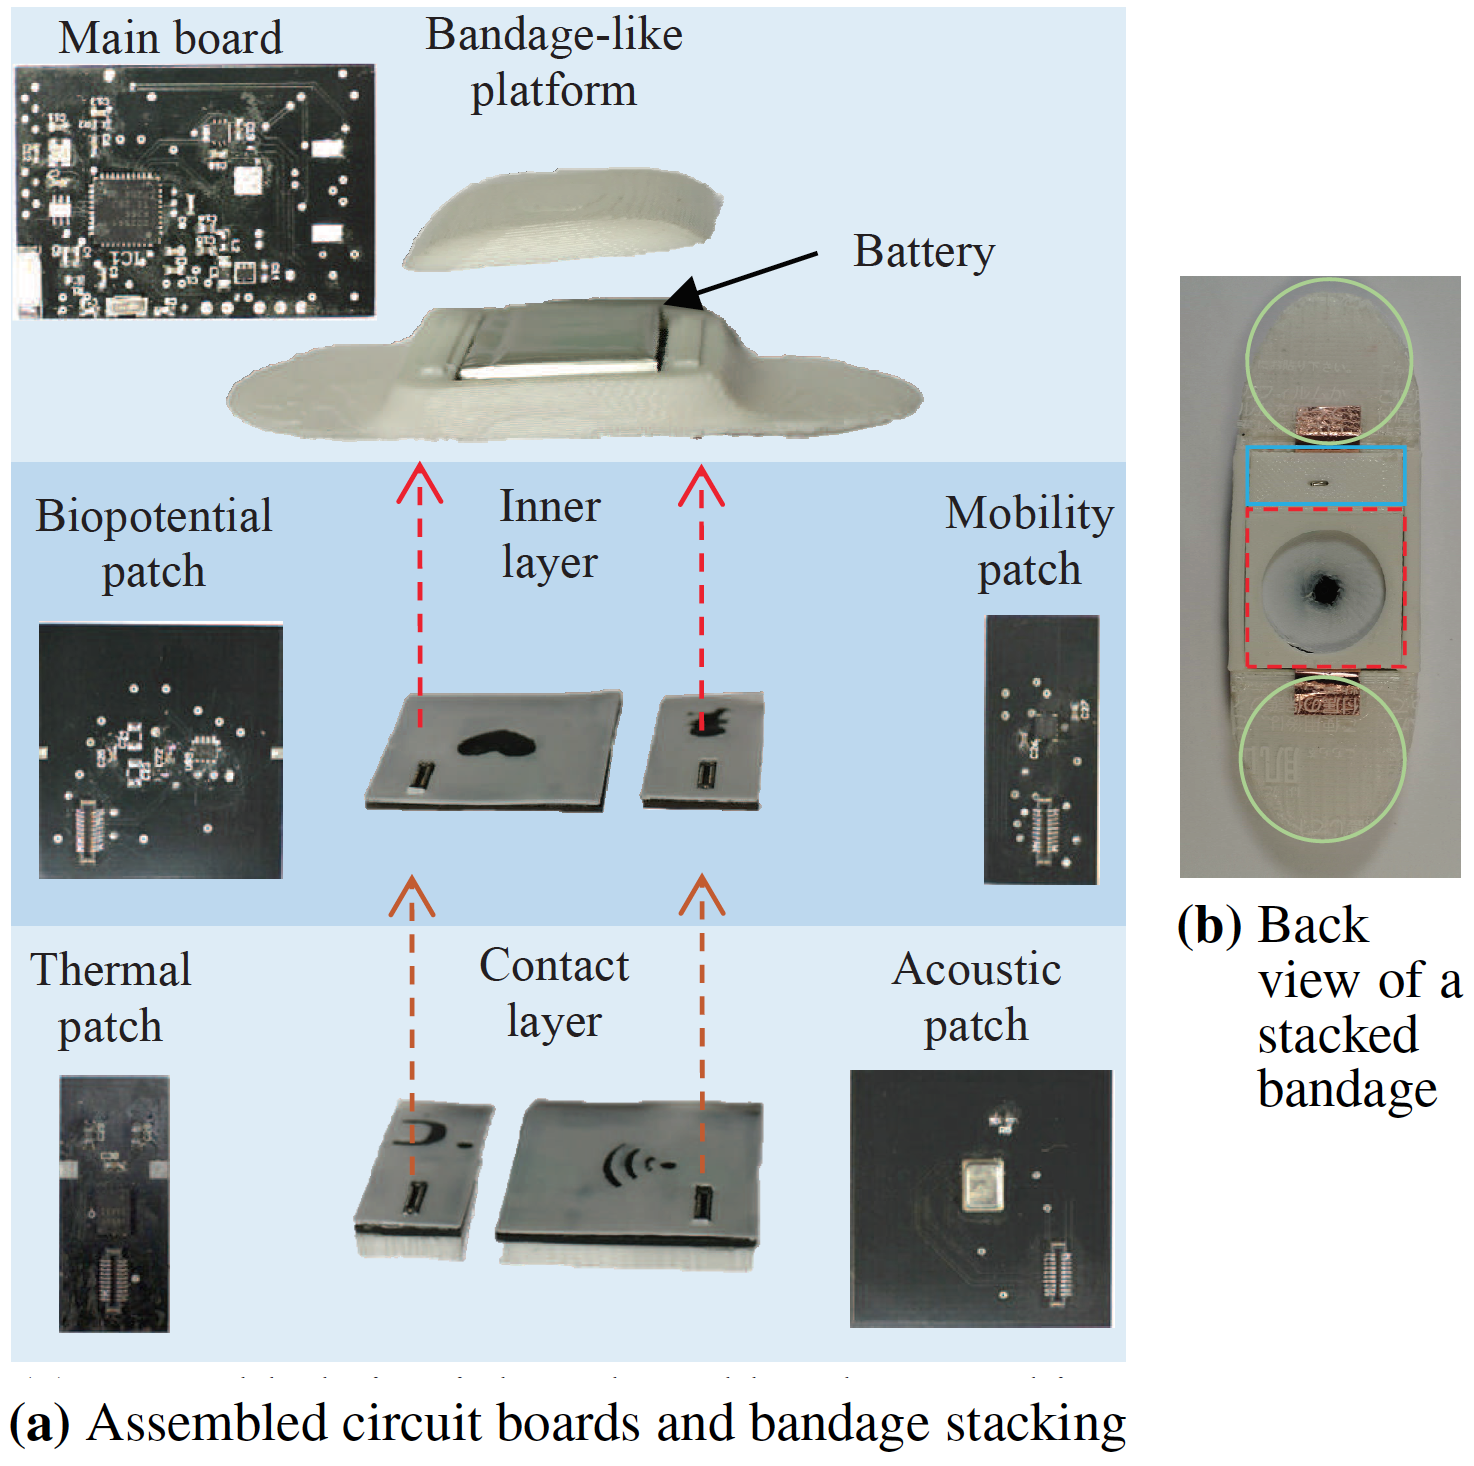
\includegraphics[width=14cm]{image/bio_fig1}
\caption{Design of the extensible sensing bandage. (a) Four patches with distinctive embossed icons are stacked on the inner and contact layers according to the direction indicated by the red dotted arrows. (b) The sound-collecting structure (box with red dashed border), a thermocouple wire (box with blue solid border), and two electrodes coated with a conductive gel (two green circles) directly contact the skin.}
\label{bandage_stacking}
\end{figure}


\subsection{Flexible and Extensible Sensing Bandage}
To create an extensible system, we designed a device with two distinct modules (Figure \ref{bandage_stacking}): (1) the basic bandage platform and (2) sensor patches. The bandage-like platform resembles an adhesive bandage. We drew a 3D model of the platform and then printed it using a 3D printer and elastic filaments. Figure \ref{bandage_stacking}(a) depicts the platform, in which a hollow space is reserved to encase the customized sensing patches. To provide processing and communication capabilities, we designed a customized circuit board, called the main board, that could be mounted in the hollow space. The main board and the stacked sensor patches are powered by a 130-mAh Li-ion battery situated in the upper layer of the platform. On the main board, a Microchip PIC32MX150 microcontroller receives data from the sensor patches through board-to-board connectors, and then relays the processed data to the monitoring screen through a Texas Instruments CC2451 Bluetooth module. \vspace{20pt}

\begin{figure}[!ht]
\centering
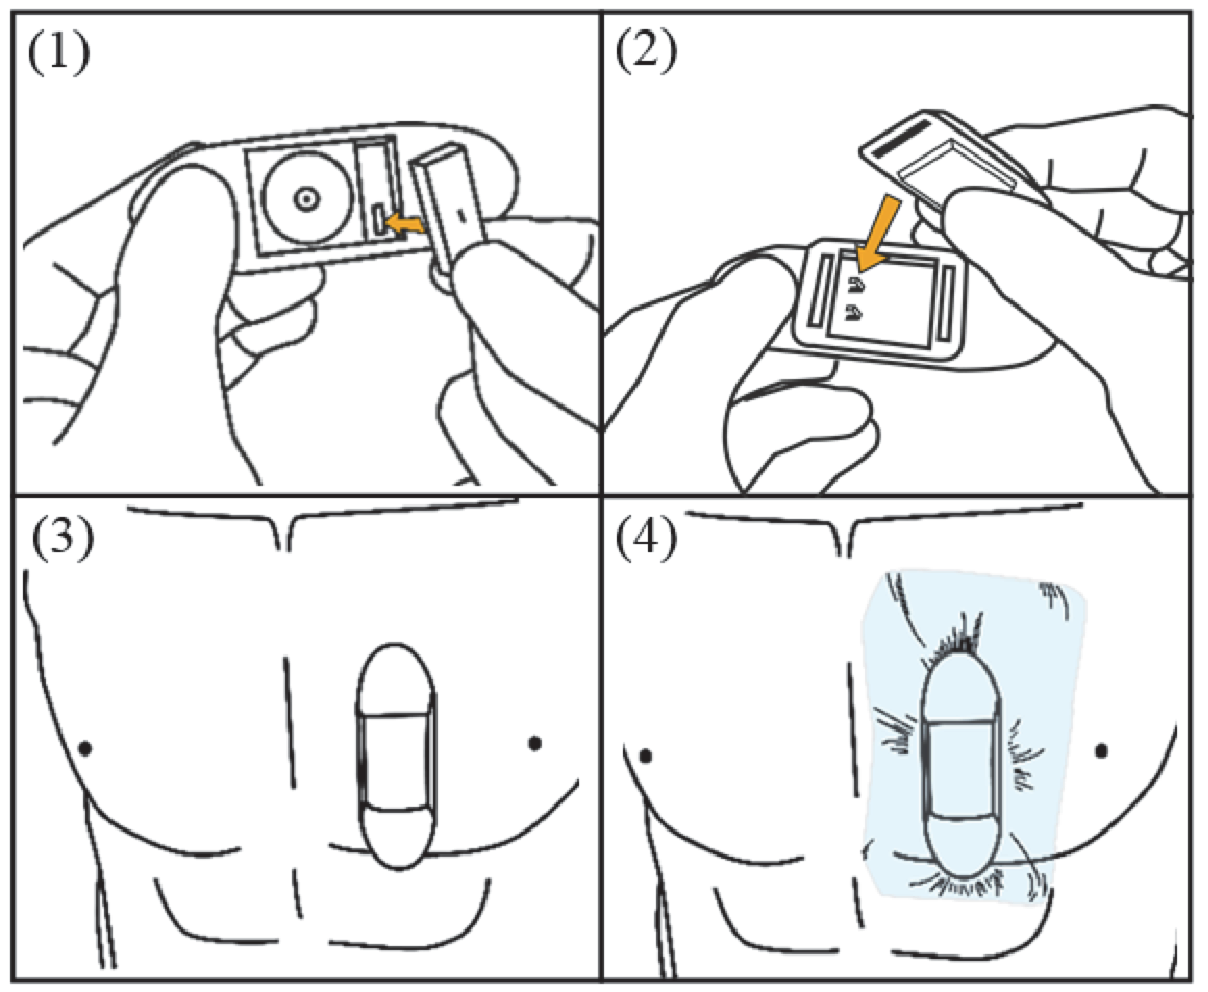
\includegraphics[width=15cm]{image/bio_fig2}
\caption{Four steps for applying bandages.}
\label{bio_steps}
\end{figure}

\subsection{Stacking Mechanism}
Users can choose different combinations of LEGO-like sensing and interaction blocks and assemble them inside a bandage form factor. This subsection describes the three main parts in stacking mechanism to make this system flexible and extensible.

\vspace{15pt}
\textbf{Assembling:}
\newline
Figure \ref{bandage_stacking}(a) illustrates these patches stacked in two layers in the hollow space of the platform; temperature and microphone sensors directly contact the skin to collect high-quality signals. 
To create accessible patches for the users, each patch was punched with a representative icon on both sides of the covering material. Figure \ref{bio_steps} illustrates the BioScope application process: (1) A healthcare worker selects the appropriate patches (or dummy patches) by using the embossed icon as a reference, stacks the patches on (or filling in empty spaces that are originally occupied by unused patches on) the platform, (2) inserts a battery and closes the protection cap, (3) affixes the bandage to chest, and (4) covers the entire bandage with transparent film dressings if water-proof is needed.
\vspace{15pt}
\begin{figure}[ht]
\centering
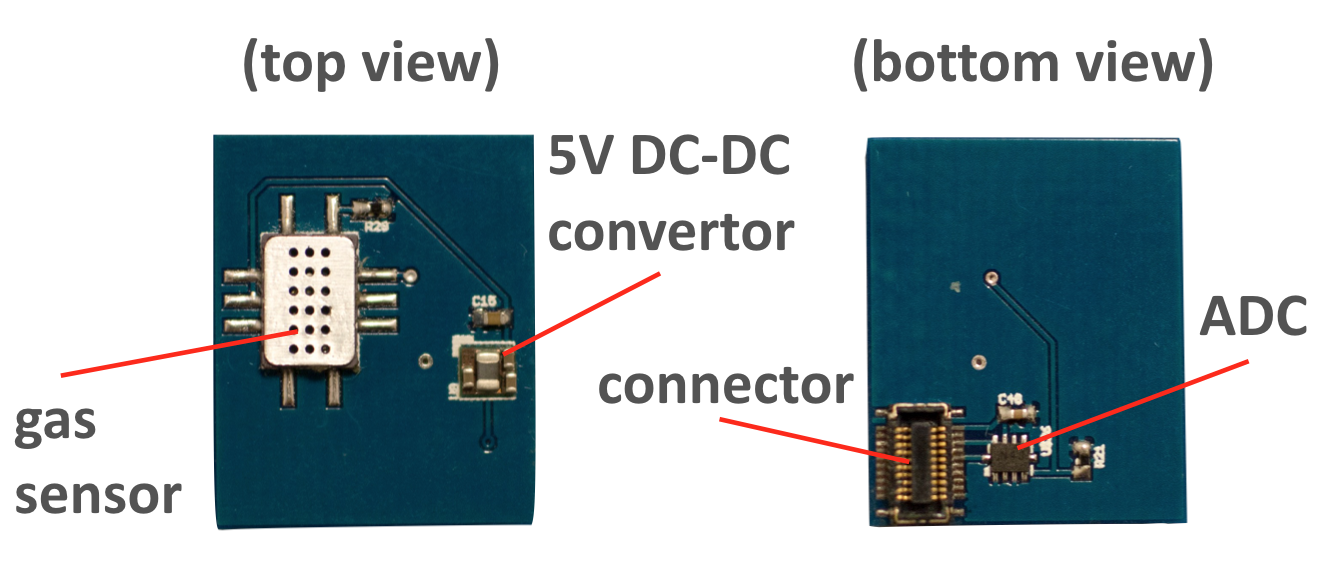
\includegraphics[width=15cm]{image/bio_dc_adc}
\caption{An example of using BioScope to prototype a breathalyzer.}
\label{dc_adc}
\end{figure}
\vspace{5pt}

\vspace{10pt}
\textbf{Power source:}
\newline
Each component in the system has different power supply range. Since  a component may require a supply voltage higher or lower than the voltage from li-ion battery (4.2V), the voltage of power source should be converted to proper voltage. A linear regulator can be used for the component, the working voltage of which is lower than the power source in the system. If the supply voltage of a component is higher than power source, a DC-DC converter can converts the voltage to a higher voltage. In figure \ref{dc_adc}, the supply voltage of the gas sensor is 5V which is higher than the voltage of the battery. Therefore, we place a compact DC-DC convertor, a Texas Instruments TPS81256, to boost the voltage to 5V and provide sufficient current to enable the sensor.

\vspace{10pt}
\textbf{Data communication:}
\newline
For a sensor that communicate to the microcontroller through digital bus, I2C and SPI are two most common protocols. Those protocols is bus topology that allows microcontroller can access multiple slave components with only few pins. However, some sensors are designed to output analog signals to deliver sensory data rather than digital signals. In Figrue \ref{dc_adc}, a Texas Instruments ADS1114 analog-to-digital converter translates the analog signals from gas sensor to digital signals in I2C.

\subsection{Sensor Patches}
To collect biosignals, such as electrocardiogram (ECG) signals, two pre-allocated electrodes (i.e., two conductive copper areas situated 6.4 cm apart at opposite ends of the bandage) are coated with a thin layer of electrical gel (Figure \ref{bandage_stacking}(b)).
The sensor patches, consisting of small sensor boards sandwiched between two thin layers of 3D-printed elastic filaments, are mounted on the bandage-like platform using connectors. To demonstrate the concept of this system, we designed six types of patch — biopotential, thermal, acoustic, mobility, interaction and recharging patches — to facilitate the collection in the most commonly monitored data in healthcare applications.
The detail of those six types of patch are described in follows.
\vspace{15pt}
\newline 
\textbf{Biopotential patch:}
\newline
This 23 mm × 24 mm patch, stacked in the inner layer, amplifies and filters ECG signals to enable continual cardiovascular monitoring. Cardiac activity, which can be characterized by ECG signals, is a crucial biosignal for assessing the cardiac functions of people. By amplifying the electrical potential difference measured between the two electrodes by using a Texas Instruments ADS1115 analog-to-digital converter on the patch, ECG signals can be monitored by allowing the passing of low-frequency signals from 0 to 100 Hz \cite{shaikh1995} by using a low-pass filter. A pulse can be identified by detecting spikes in the signal, thus enabling users to assess heart and respiratory rates.
\vspace{10pt}
\newpage
\textbf{Acoustic patch:}
\newline
This 24 mm × 24 mm patch, stacked in the contact layer, records acoustic signals emitted by a person's body or while the person is phonating. By identifying the unique sound patterns that the body's organs generate, users can assess person's conditions. Furthermore, person's phonation can indicate social interaction, according to which users can assess whether a person is depressed or impaired cognitively.  To clearly record the internal sounds of the body, a mediating instrument (e.g., a stethoscope) is required. Inspired by the design of electronic stethoscopes, we designed and attached a small sound-collecting structure (Figure \ref{bandage_stacking}(b)) on the patch that effectively amplified acoustic signals from the body and occluded environmental noise. Above the sound-collecting structure, an opening is aligned with the receiving hole of an InvenSense INMP441 microphone on the main board to guide sound waves towards the hole. In this study, we detected a person phonation, which reflected social activity, by analyzing the frequency components of the collected sound.
\vspace{10pt}
\newline
\textbf{Thermal patch:}
\newline
This 10 mm × 24 mm patch is stacked in the contact layer and measures the skin temperature, which can indicate a person's health. users can evaluate a person by identifying abnormal or varying temperatures \cite{Freitas1999}. A Maxim MAX31850 K-type thermocouple-to-digital converter detects body temperature through a thermocouple wire that protrudes from the covering elastic material to contact the skin of the person (Figure \ref{bandage_stacking}(b)).
\vspace{10pt}
\newpage
\textbf{Mobility patch:}
\newline
This 11 mm × 24 mm patch, stacked in the inner layer, monitors the mobility level of a person. For example, to prevent complications caused by reduced mobility levels and assess functional recovery, users must track the mobility level of patients. On this patch, a Bosch BMA250 accelerometer is used to collect acceleration readings, which indicate whether a person is moving or stationary. The mobility level can be derived by calculating the percentage of time a person is moving.
\vspace{10pt}
\begin{figure}[ht]
\centering
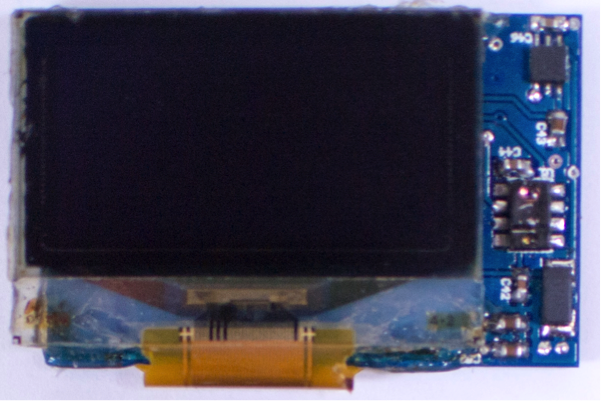
\includegraphics[width=12.5cm]{image/bio_fig1_5}
\caption{Interaction patch.}
\label{interaction_patch}
\end{figure}
\newline
\textbf{Interaction patch:}
\newline
To enrich data feedback and user interaction for exercise applications, we also expanded an interaction patch that consists of a wearable display (0.96” OLED display4), and a touchless gesture sensor (Avago APDS-9960) that is used to recognize four directions (up, down, left and right) of in-air swipe gesture. The gesture can be used to switch between different sensor's data or different data representations as shown in Figure \ref{interaction_patch}. The interaction patch is connected to main board through stacking mechanism as well. When a mobile device attempts to establish connection with particular one of multiple wearable devices. To simplify Bluetooth pairing procedure for quickly retrieving data or configuring device, a NXP NTAG203 NFC tag is embedded in wearable device.
\vspace{10pt}
\begin{figure}[ht]
\centering
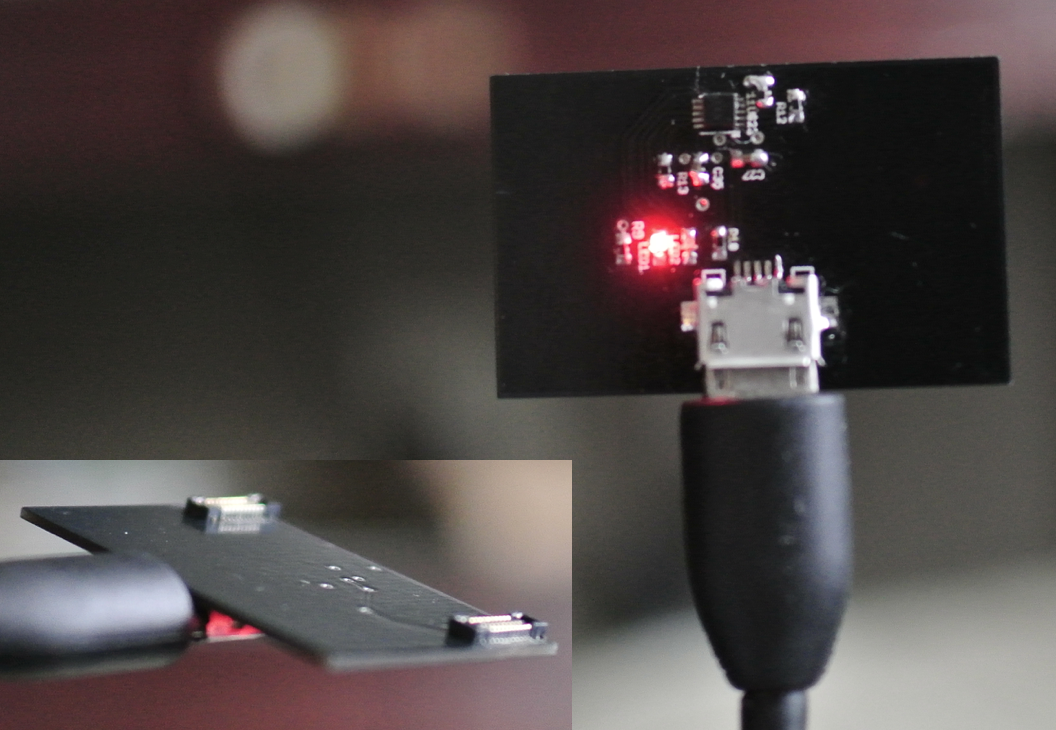
\includegraphics[width=13cm]{image/bio_recharge}
\caption{Recharging patch.}
\label{bio_recharge}
\end{figure}
\newline
\textbf{Recharging patch:}
\newline
The entire system is powered by a Li-ion battery with 130-mAh capacity. This patch has a USB connector to connect a 5V power source for charging and a Texas Instruments BQ24040 to regulate the voltage in charging process (Figure \ref{bio_recharge}).


\subsection{Explorative Experiment}
To validate system functionality, we scripted a sequence of activities to simulate conditions arising when a patient with basic functional mobility is hospitalized. Two volunteers performed the specific activities while wearing bandages equipped with all four patches on their chests, enabling us to collect data (Figure \ref{bio_exp_result}(a)). The simulations were con- ducted for 10 and 30 minutes in the cases of the first and second participants (P1 and P2), respectively. Activities comprised (1) lying down on a bed, (2) having a phone conversation, (3) watching TV, (4) having a face-to-face conversation, and (5) performing walking. In the experiments, the data captured were heart rate, skin temperature, received acoustic signals, and mobility indicators.

Figure \ref{bio_exp_result}(b) shows the results obtained by analyzing the data collected from P1. The readings obtained from the mobility patch indicated that P1 moved between the seventh and ninth minutes; this was an accurate assessment of the patient's behavior during that time. While walking, P1's heart rate increased relative to that while stationary between the start and the seventh minute. When the posture of the patient drastically changed, such as when P1 stood up near the second, seventh, and ninth minutes, the ECG signals were distorted \cite{chan2013}, producing a dip in the calculated heart rate. The sounds generated by clothes rubbing against the bandage when P1 moved adversely affected the quality of detected internal sounds, causing the amplitudes to increase between the seventh and ninth minutes. After filtering out sounds generated by movement, however, we could still detect when P1 phonated between the second and seventh minute. Based on the vocal resonance of the body \cite{Dacre2002}, we detected phonation by identifying the frequency components of sounds higher than the 0- to 3-kHz frequency range of the human voice [7]. Finally, the body temperature varied minimally (34$^{\circ}$C $\sim$ 35$^{\circ}$C) and was near the normal skin temperature of the human chest \cite{Freitas1999}. Overall, the results accurately reflected the activities performed by the participants.

To examine whether the system can detect reasonable values for the average heart rate, total moving duration, average skin temperature, and total phonating time, we analyzed the data collected from P2 over 30 minutes. The total moving duration was determined to be 7.2 minutes (actual value: 6.9 minutes), with an error of 4.0\%. The average heart rate was 81.5 and 100.3 beats respectively.  Because P2 did not perform intensive exercise, the average temperature did not vary significantly, remaining near 33.9◦C. By identifying the high-frequency components embedded in the high-pitched sounds collected when P2 was stationary, P2 was deter- mined to have phonated for 635.5 seconds (actual value: 564.0 seconds), with an error of 12.7\%. per min (BPM) when P2 was stationary and moving, respectively.  Because P2 did not perform intensive exercise, the average temperature did not vary significantly, remaining near 33.9◦C. By identifying the high-frequency components embedded in the high-pitched sounds collected when P2 was stationary, P2 was deter- mined to have phonated for 635.5 seconds (actual value: 564.0 seconds), with an error of 12.7\%.

\begin{figure}[!ht]
\centering
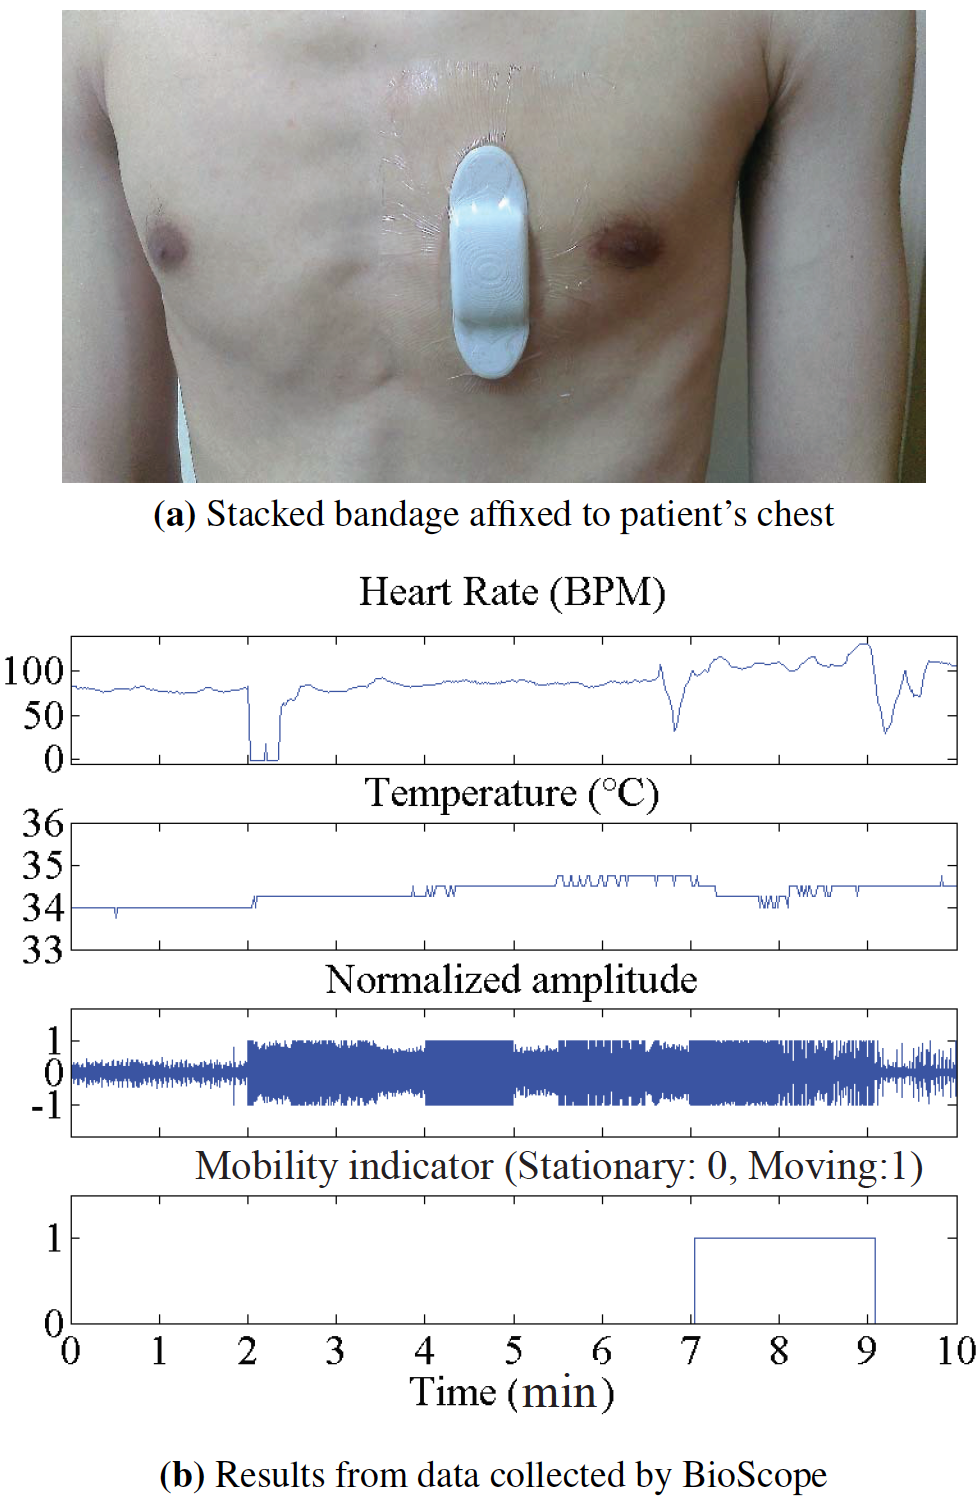
\includegraphics[width=12cm]{image/bio_fig4}
\caption{Four steps for applying bandages.}
\label{bio_exp_result}
\end{figure}


%\section{Configuration}

%\section{Application programming interface}

\section{...}


\section{...}


\chapter{Conclusion}






\let\cleardoublepage\clearpage

\appendix
\chapter{Sensor-Embedded Teeth for Oral Activity Recognition}

The human mouth is one part of the human body that is almost always in constant use. We use our mouth to perform some of the most important daily functions, such as eating, drinking, speaking, coughing, breathing, and smoking. Because our mouth is an opening into assessing the health of the human body, it presents the opportunity for the placement of a strategic sensor for detecting human oral activities. For this study, we developed such an oral sensory system, where we explored the use of a small motion sensor embedded inside artificial teeth for the recognition of human oral activities. The detection of human oral activities can enable numerous health care applications, such as food and fluid intake monitoring.   
Previous research has explored wearable sensory devices installed in various locations of the upper body for detecting human oral activities. For example, Amft et al. [1] used an earphone-attached microphone sensor to record human chewing sounds and detect food types based on their acoustic profiles. Amft et al. [2] proposed another approach that combined surface Electromyography (EMG) and a microphone worn around the neck area to recognize low- or high-volume swallowing actions. BodyScope [3] placed an acoustic sensor around the neck area to recognize different oral activities (e.g., eating, drinking, speaking, laughing, and coughing) by analyzing sounds generated from the throat area. In comparison, our oral sensory system explores a unique sensor placement not on the human body, but inside the human body, specifically the mouth. Because a sensor placement inside the mouth has the advantage of being in proximity to where oral activities actually occur, this enables our oral sensory system to accurately capture the motion of oral activities. 
This paper presents the design and evaluation of this in-mouth oral sensory system, which uses a small accelerometer sensor embedded inside artificial teeth. Our motivation was based on our observation that most oral activities, such as chewing, drinking, speaking, and coughing, each produce a unique teeth motion. By recording and identifying teeth motion profiles for each oral activity, the proposed oral sensory system builds classifiers that distinguish different human oral activities. 

\begin{figure}[!ht]
\centering
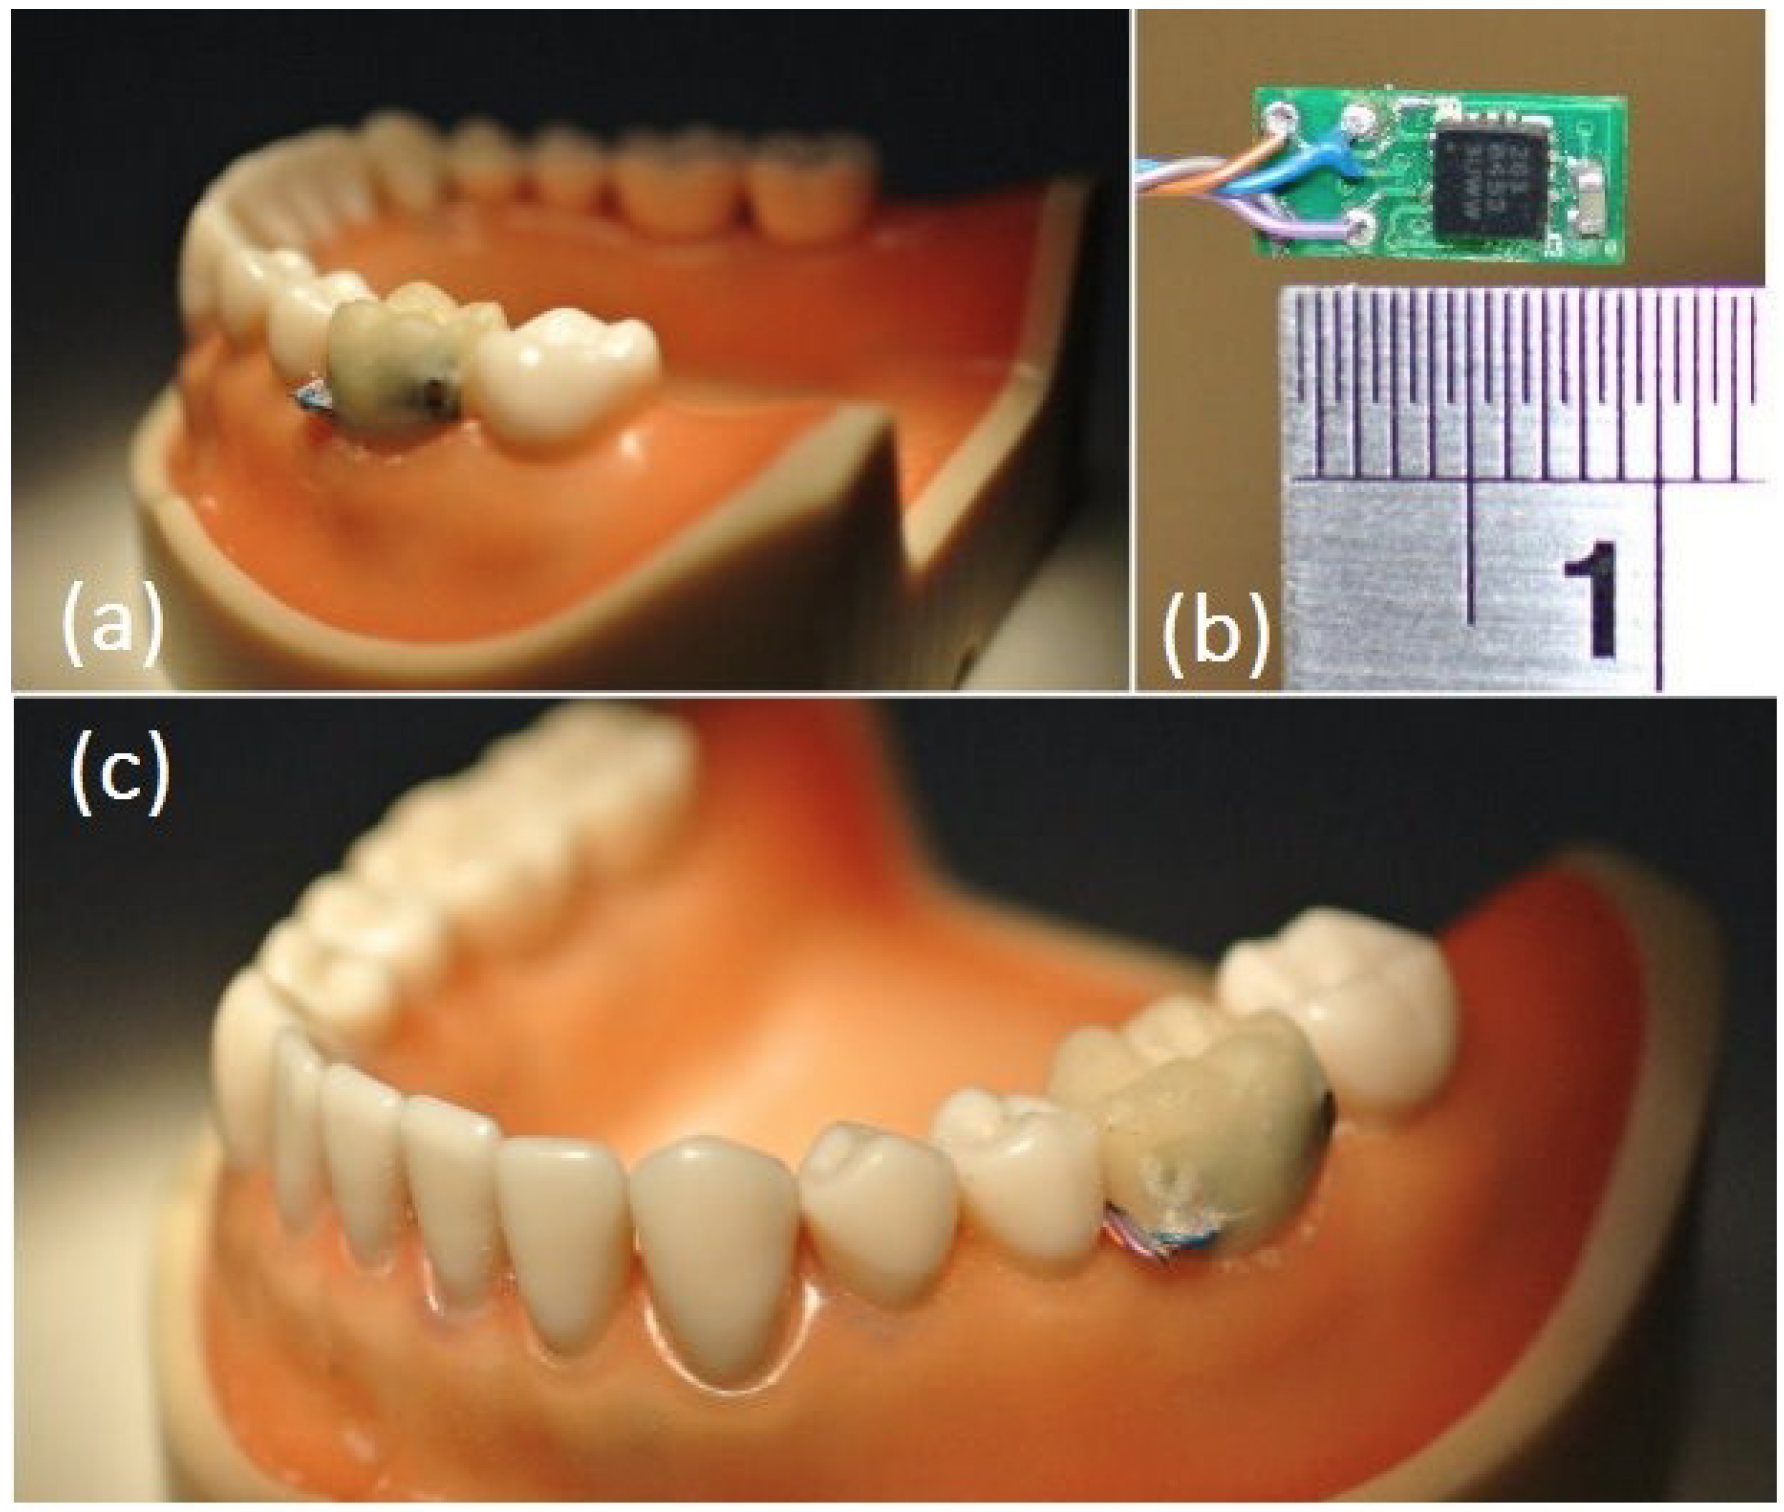
\includegraphics[width=14cm]{image/teeth}
\caption{The breakout board with (b) tri-axial accelerometer and (a)(c) sensor embedded denture.}
\label{teeth_overview}
\end{figure}

\section{System Overview}
The system consists of two main components: (a) an oral sensory unit; and (b) oral activity classifiers. 

\subsection{Oral Sensory Unit}
Figure 1(b) shows a small breakout board with a tri-axial accelerometer sized 4.5 mm x 10 mm. This small breakout board is sufficiently small to be embedded inside a removable artificial tooth, as shown in Figs. 1(a) and 1(c). To ensure that this sensor board is safe and saliva-proof for human mouth placement, we carefully coated the sensor board with dental resin. In actual system deployment, this sensor board would include a small Bluetooth radio capable of wirelessly transmitting sensor data to a nearby mobile phone for data analysis and oral activity recognition. In the current proof-of-concept system, we have yet to place a Bluetooth radio on this oral sensory unit; therefore, thin wires are used to connect the sensor board to an external data-logging device for data retrieval and power. These thin wires also protect users from accidentally swallowing the sensor units. 
Oral Activity Analysis
Oral activity recognition comprises the following three steps: (1) data preprocessing, (2) feature extraction, and (3) data classification. These steps are described as follows: 
\subsubsection{Data preprocessing}
The sampling rate of the accelerometer sensor is set to 100 Hz. The system first divides the accelerometer data into windows of 256 samples with a 50\% overlap between consecutive windows \cite{KristofVanLaerhoven:2000}. In each data window, the system extracts the time-domain and frequency-domain features shown in Table \ref{teeth_features}. 
Because people have different mouth and teeth specifications, sensor orientation can change for different users. Thus, accelerometer readings must be adjusted and calibrated using a rotation matrix. During the calibration phase, the proposed system asks users to hold their head straight and still for a few seconds during the application of Rodrigues' rotation formula to compute this rotation matrix. Each oral sensor unit has its own rotation matrix, which is used to transform its sensor readings from the device's coordinates to real-world coordinates. This normalization procedure reduces the negative effect of errors caused by varying device orientation. Because this normalization procedure reduces, but does not completely remove this error, the system also extracts orientation-independent features based on the magnitudes of x-, y-, and z-axis acceleration. For each sample at time t, its magnitude data is calculated as $\sqrt{x_{t}^{2}+y_{t}^{2}+z_{t}^{2}}$.


The normalized (orientation-dependent) feature set and the orientation-independent feature set have different characteristics. The normalized feature set retains separate information on tri-axial acceleration values, which are required for distinguishing activities involving both vertical and horizontal movements. In contrast, the orientation-independent feature set is based on the magnitude value, in which its precision is less affected by changes in device orientation; thus, it is suitable for distinguishing activities that depend on the movement scale.

\subsubsection{Feature extraction}
Table \ref{teeth_features} lists the time-domain and frequency-domain features extracted from each data window. Frequency-domain features are computed using the FFT algorithm. Both real and imaginary components of FFT coefficients in the 256-sample window are used to generate 256 features. Overall, the system trains activity classifiers by computing and extracting the following two feature sets: 807 features (269 features per axis acceleration) from the normalized feature set, and 269 features from the device-independent feature set.

\begin{table*}[!ht]
\centering
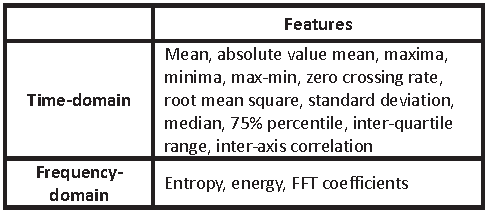
\includegraphics[width=14cm]{image/teeth_table1}
\caption{Adopted features for oral activity recognition.}
\label{teeth_features}
\end{table*}

\subsubsection{Training Classifiers}
Our system implements three classifiers: the C4.5 Decision Three (DT), the Multivariate Logistic Regression (MLR), and the Support Vector Machine (SVM). The SVM classifier uses the radial basis function kernel and one-against-one multiclass classification, and it is further optimized by an additional parameter selection and data scaling. To filter out redundant and irrelevant features, we performed feature selection based on the correlations between features. Low-relevance features with low correlation are filtered out. We adopted principal component analysis [5] as a feature selector, in which the number of relevant features was reduced to 137. 
For each classification algorithm of the DT, the MLR, and the SVM, we trained two classifiers: person-dependent and person-independent. A person-dependent classifier uses data from all users (i.e., 8 participants in our study) to train a generalized activity model for recognizing the oral activities of different users. Conversely, a person-independent classifier uses 7 users' data to train a specify activity model for recognizing remaining person's oral activities.

\section{Experimental Evaluation}
We conducted a laboratory experiment to evaluate the accuracies of different classification algorithms.

\subsection{Experimental Procedure}
Eight users (5 males and 3 females) participated in this experiment. They were asked to install the oral sensor unit inside their mouth while performing each of these four oral activities: chewing, drinking, talking, and coughing. Because it was not possible to customize a removable tooth for each participant, we used dental cement to fix the sensor units to each participant's tooth. For each activity, we collected 15 samples from each participant. Each sample consisted of 2.56 seconds of a specific activity performance. For the coughing data, participants were asked to cough continuously. For drinking data, participants were asked to drink a bottle of water. For chewing data, participants were asked to chew gum or to imitate the action. For speaking data, participants were asked to read a section of an article. We collected 480 activity samples from the 8 participants performing these four oral activities. Person-dependent and person-independent classifications used the same data set collected from the experiment.

\subsection{Results}
We conducted 10-fold cross-validation and leave-one-person-out cross-validation to measure the accuracies of the person-dependent and person-independent classifiers. For the person-dependent classifiers, each round of cross-validation involved using all of each participant's data for both training and testing. Table \ref{teeth_pdc} shows the mean F-measure accuracy results. The SVM (93.8\%) classifier outperforms both the DT (52.2\%) and MLR (60.5\%) classifiers.  

For the person-independent classifiers, each round of cross-validation involved using 7 participants' data for training, and the remaining participant's data for testing. Table \ref{teeth_pdc} shows the mean F-measure accuracy results. Again, the SVM (59.8\%) classifier outperformed both the DT (40.8\%) and MLR (55.9\%) classifiers. Reasons for the low-accuracy result in the person-independent classifier are as follows.
First, because people's teeth and mouth structure are different, their sensor placements are also (slightly) different, thus creating variations in the motion data. Second, people perform oral activities differently; for instance, some people chew or talk faster, slower, harder, or softer. It is possible to improve the accuracy of person-independent classification by extending the training set to include different sensor placements and oral activity types.
\newpage

\begin{table*}[!ht]
\centering
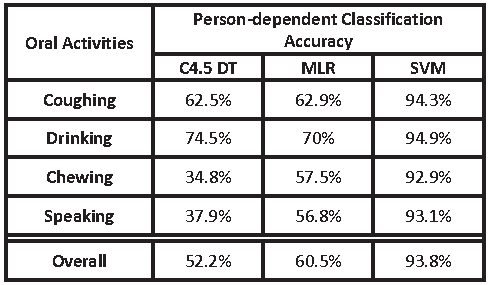
\includegraphics[width=14cm]{image/teeth_table2}
\caption{F-measure accuracy of oral activity recognition with a person-dependent classifier.}
\label{teeth_pdc}
\end{table*}

\begin{table*}[!ht]
\centering
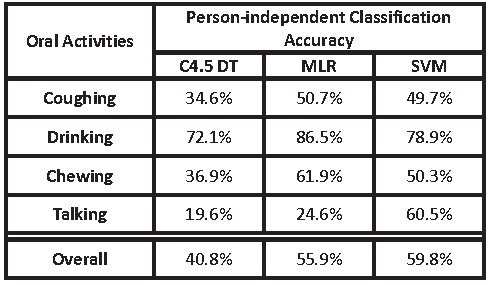
\includegraphics[width=14cm]{image/teeth_table3}
\caption{F-measure accuracy of oral activity recognition with a person-independent classifier.}
\label{teeth_pidc}
\end{table*}

\newpage
\section{Discussion}
This is a feasibility study of an oral sensory system that detects human oral activities. We identified the following challenges for the proposed oral sensory system.

\subsubsection{Data logging and transmission}
If an application does not require real-time monitoring, sensory data can be temporarily stored on the sensor device. When users remove their artificial teeth, for example, for disinfection and storage, small electrodes on the surface of the artificial teeth are used to connect to the sensor board and retrieve stored sensor data. For a real-time monitoring application, the sensor board must have a low-power wireless radio (e.g., Bluetooth) to transmit sensor data to a nearby smartphone for data analysis and activity recognition. Another possible data transmission medium is intra-body communication \cite{Hachisuka:2003}, which has lower power consumption compared to wireless radio communication.

\subsubsection{Energy}
Because users must remove artificial teeth for daily disinfection and storage, we surmise that a recharging and storage station will be required, similar to that of an electric toothbrush, in which users would place the cleaned artificial teeth on this station for battery recharging and data retrieval. 

\subsubsection{Safety}
Because of the sensor placement inside the mouth, the safety concern is paramount. All electronic components must be sealed securely and tightly. In the event that the sensor units are mistakenly swallowed, they will pass the human body without causing any harm. Its safety requirements are similar to those of capsule endoscopy, in which patients swallow a camera pill. Because our current prototype (Figure \ref{teeth_overview}) was not considered safe, we attached a safety string to the sensor unit so that participants would not be able to swallow it.

\subsection{Summary}
For this study, we designed and developed an oral sensory system that can recognize human oral activities. Our results from a laboratory experiment with 8 participants demonstrate the feasibility of this oral sensory system in recognizing the following four human oral activities: speaking, chewing, drinking, and coughing. We found that a person-dependent SVM classifier achieved a high F-measure accuracy of 93.8$\%$, whereas a person-independent SVM classifier achieved only an F-measure accuracy of 59.8$\%$. 
Because the mouth is an opening into human health, this oral sensory system has the potential to enhance exiting oral-related healthcare monitoring applications such as dietary tracking. 

\let\cleardoublepage\clearpage


\backmatter

\addcontentsline{toc}{chapter}{\bibname}
\bibliographystyle{abbrv}

% Your bibliography goes here
\bibliography{thesis}

\end{document}
